    \documentclass[letterpaper,11pt]{article}

    \usepackage{fullpage}
    \usepackage[usenames,dvipsnames]{color}
    \usepackage[pdftex]{hyperref}
    \usepackage{tabularx}
\usepackage{booktabs}
\usepackage{amsmath}
\usepackage{multirow}
\usepackage{layouts}
\usepackage{array}
\usepackage{pgf}
\usepackage{tikz}
\usetikzlibrary{positioning}
\usetikzlibrary{arrows,automata}
 \usepackage{graphicx}

    \hypersetup{
	colorlinks,%
	citecolor=black,%
	filecolor=black,%
	linkcolor=blue,%
	urlcolor=mygreylink     % can put red here to visualize the links
    }
   
    \definecolor{mygrey}{gray}{.85}
    \definecolor{mygreylink}{gray}{.30}
    \textheight=8.6in
    \raggedbottom
    \raggedright
    \setlength{\tabcolsep}{0in}
    \addtolength{\oddsidemargin}{-0.375in}
    \addtolength{\evensidemargin}{0.375in}
    \addtolength{\textwidth}{0.5in}
    \addtolength{\topmargin}{-.375in}
    \addtolength{\textheight}{0.75in}

    \newcommand{\resitem}[1]{\item #1 \vspace{-2pt}}
    \newcommand{\resheading}[1]{{\LARGE \colorbox{mygrey}{\begin{minipage}{\textwidth}{\textbf{#1 \vphantom{p\^{E}}}}\end{minipage}}}}
    \newcommand{\ressubheading}[4]{
    \begin{tabular*}{6.5in}{l@{\extracolsep{\fill}}r}
		    \textbf{#1} & #2 \\
		    \textit{#3} & \textit{#4} \\
    \end{tabular*}\vspace{-6pt}}
  
    \begin{document}

\begin{center}
{\Large \textbf{Machine Learning: Pattern Recognition}}\\ [1em]
\end{center}
\newcommand{\mywebheader}{
    \begin{tabular}{@{}p{5.3in}p{4in}}
		{\resheading{{\LARGE Report Lab 1}}} & { {\Large 11 September, 2012}}\\\vspace{0.3cm}
	    \end{tabular}}
    \mywebheader
    
    	\begin{center}
    	{\Large By:} \\ \vspace{0.1cm}
	    {\Large Paris Mavromoustakos} \\  \vspace{0.1cm}
	    {\Large Georgios Methenitis} \\ \vspace{0.1cm}
	    {\Large Marios Tzakris}
	    \end{center}

  
  \section*{Introduction}
  The purpose of this lab assignment was to apply a k-Nearest-Neighbors classification algorithm on a given set of data-points. To achieve this we had to become familiar with the Matlab environment, including the Netlab package. The Netlab package is a complete suit of Matlab functions implementing machine learning techniques.
 
 \section*{Exercise 1}
 First of all, we loaded a given data file (\texttt{twoclass.mat}) which contained two classes of two-dimensional data points. Before creating both the training and test sets, we shuffled the two matrices in order to create groups of random data points. \textbf{The training set consists of 75\% of data points from class A appended to 75\% of data points from class B, while the test set contains the remaining 25\% of both classes A and B}. Figure~\ref{fig:1} presents the plot results of the training set. \textbf{Data points of different classes are depicted with different symbols and colors}. Figure~\ref{fig:2} presents the plot results of the test set.
 
 \begin{figure}[h!]
\centering
  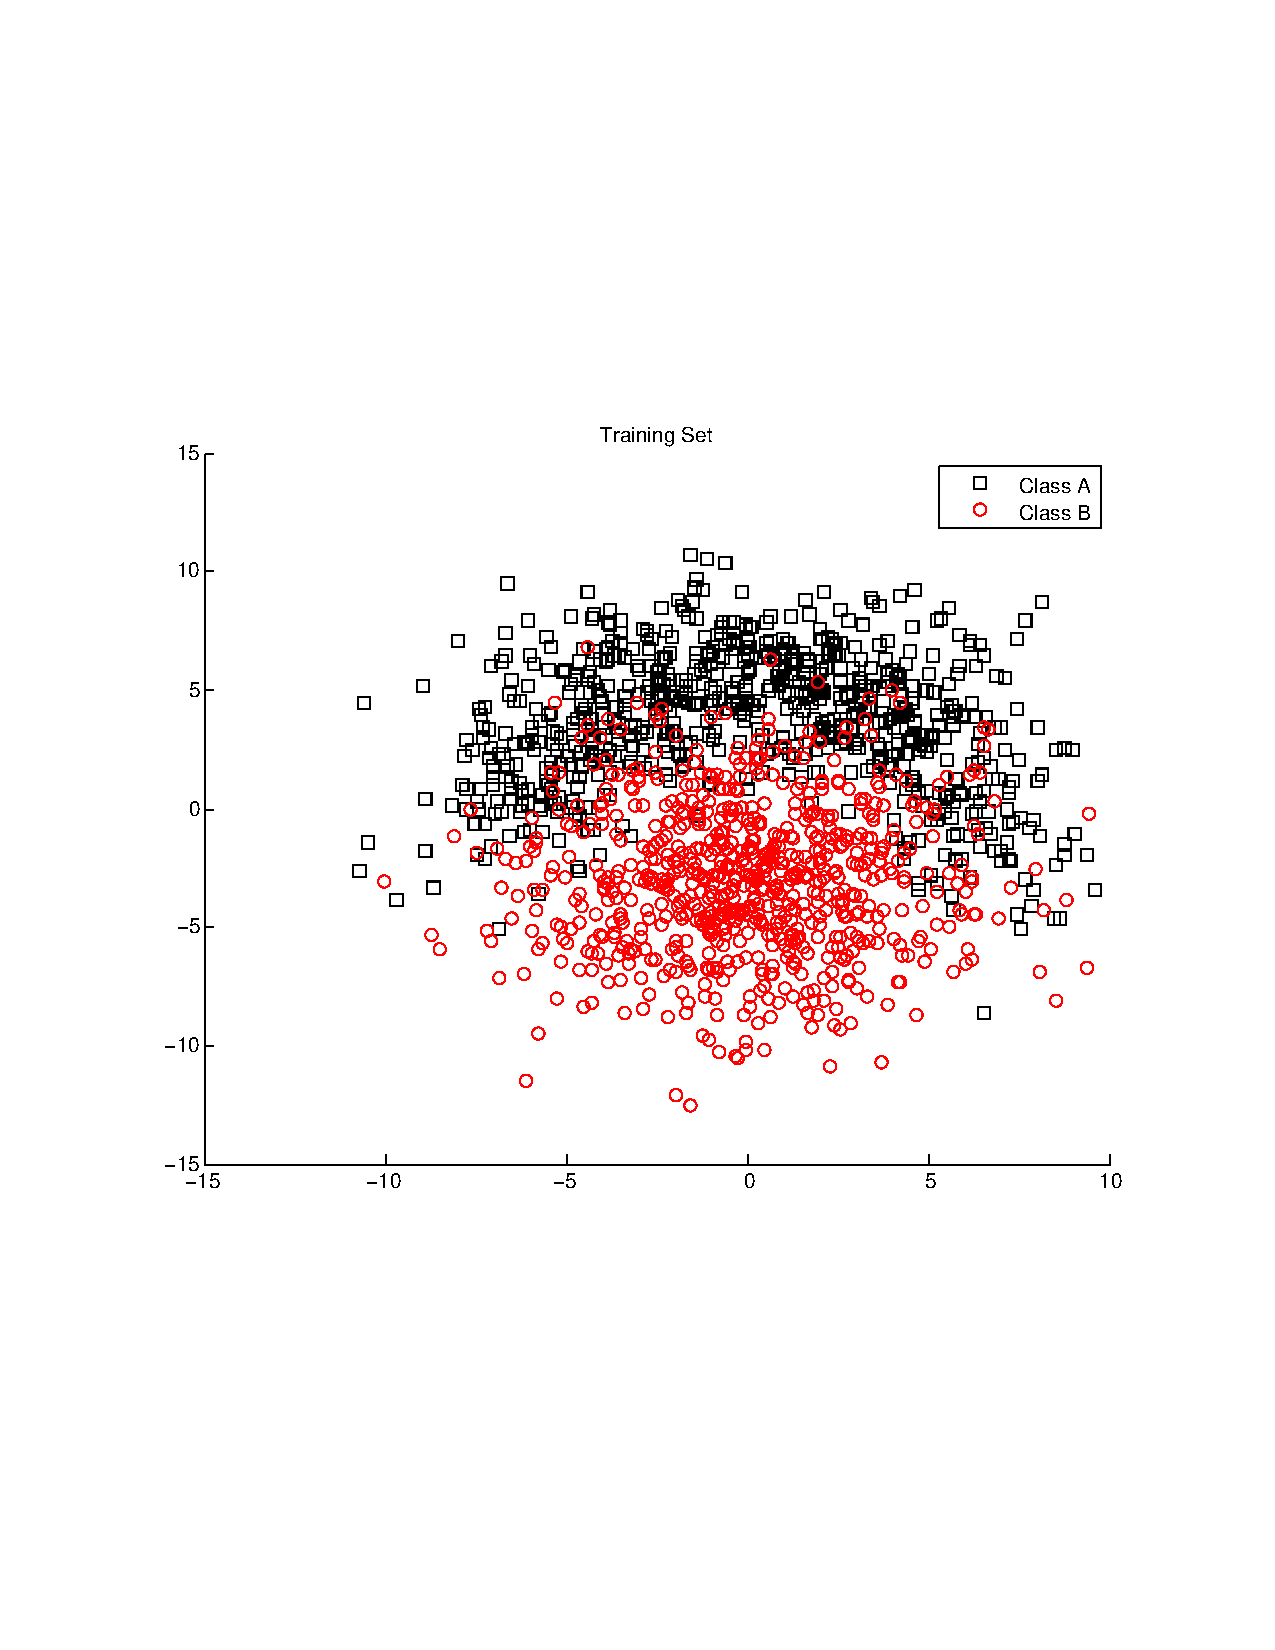
\includegraphics[trim = 0cm 7.5cm 0cm 7cm, clip, width=0.8\textwidth]{figures/TrainingSet.pdf}
  \caption{Data points of the Training Set.}
  \label{fig:1}
\end{figure}
 
  \begin{figure}[t!]
\centering
  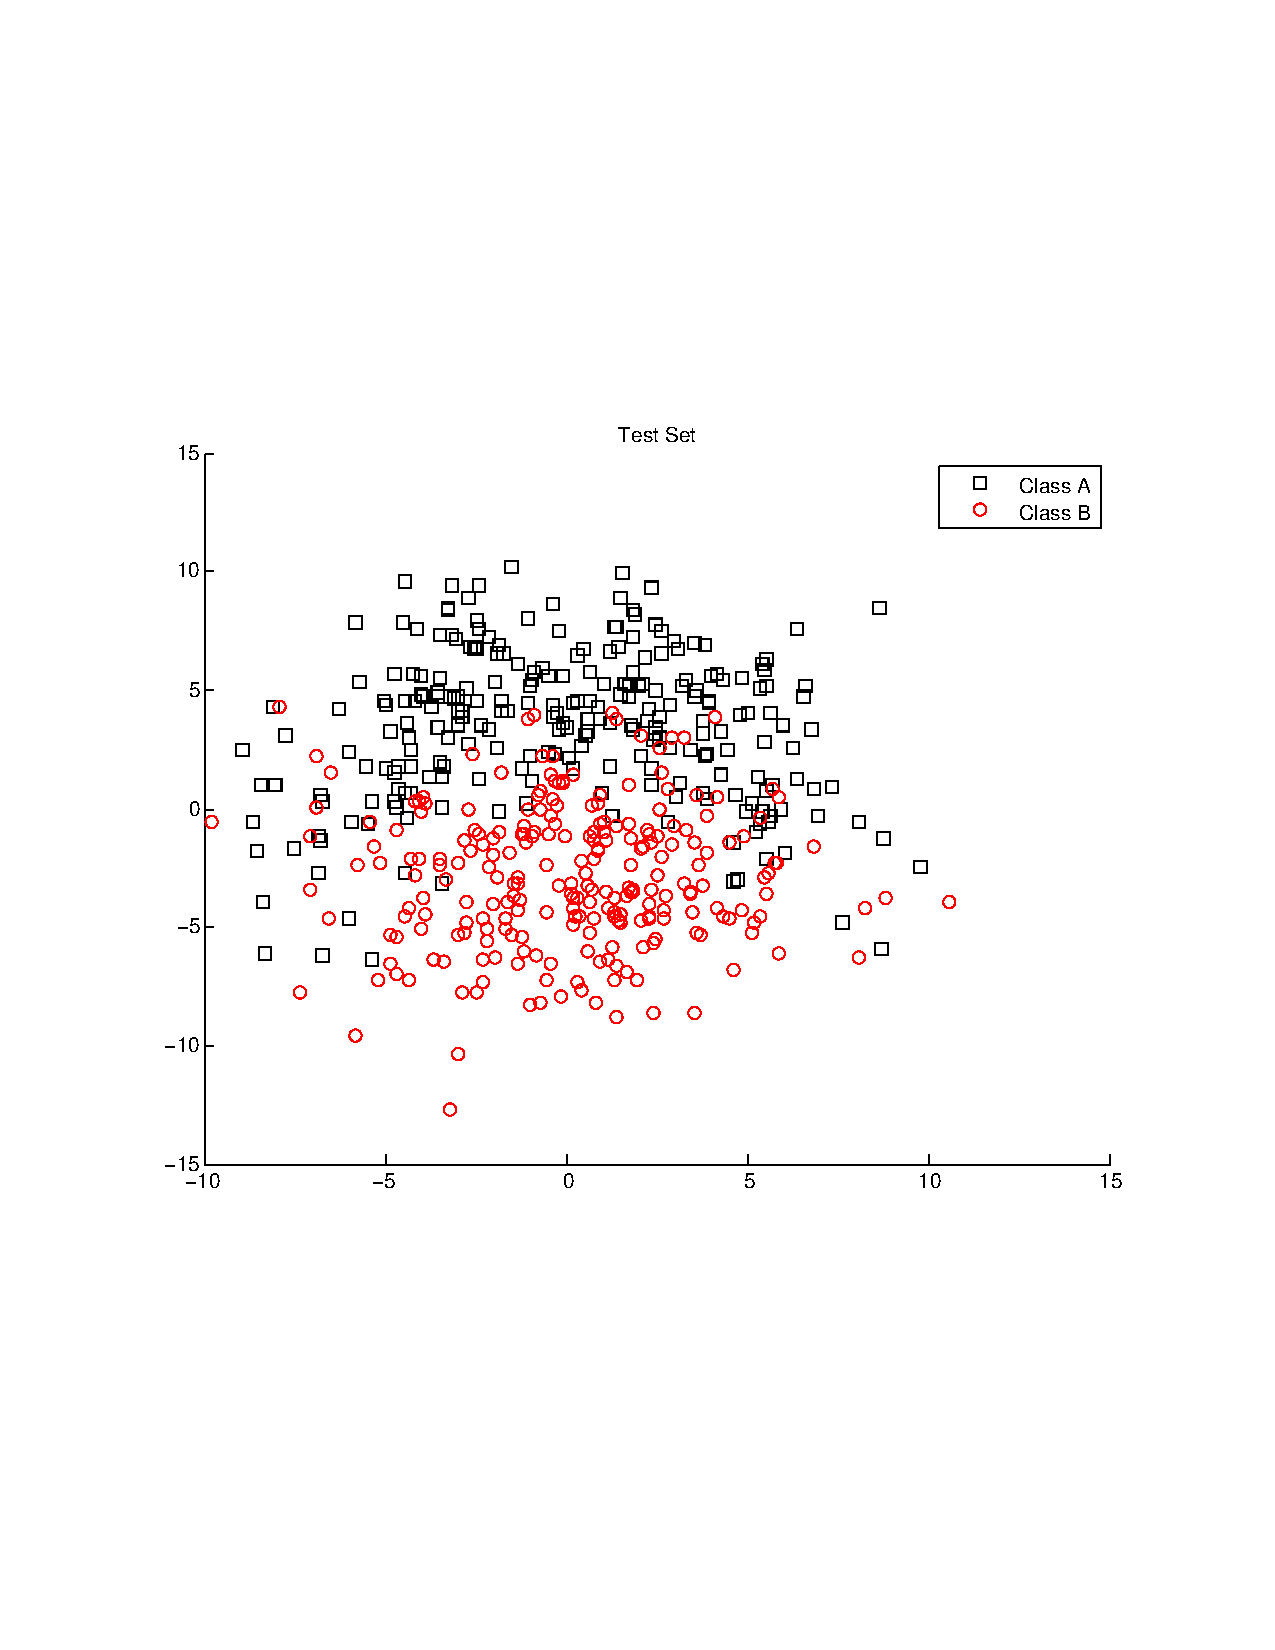
\includegraphics[trim = 0cm 7.5cm 0cm 7cm, clip, width=0.8\textwidth]{figures/TestSet.pdf}
  \caption{Data points of the Test Set.}
  \label{fig:2}
\end{figure}



\section*{Exercise 2}
We trained our knn classifier using the training data, evaluating its performance on the test data and computing the misclassification rate. The misclassification rate taking into consideration only one neighbor (k=1) is $17\%$. Then we tried several odd values for k ($k=1, 3, 5, \ldots, 29$), computing the error for each case as shown in Figure~\ref{fig:3}.


  \begin{figure}[h!]
\centering
  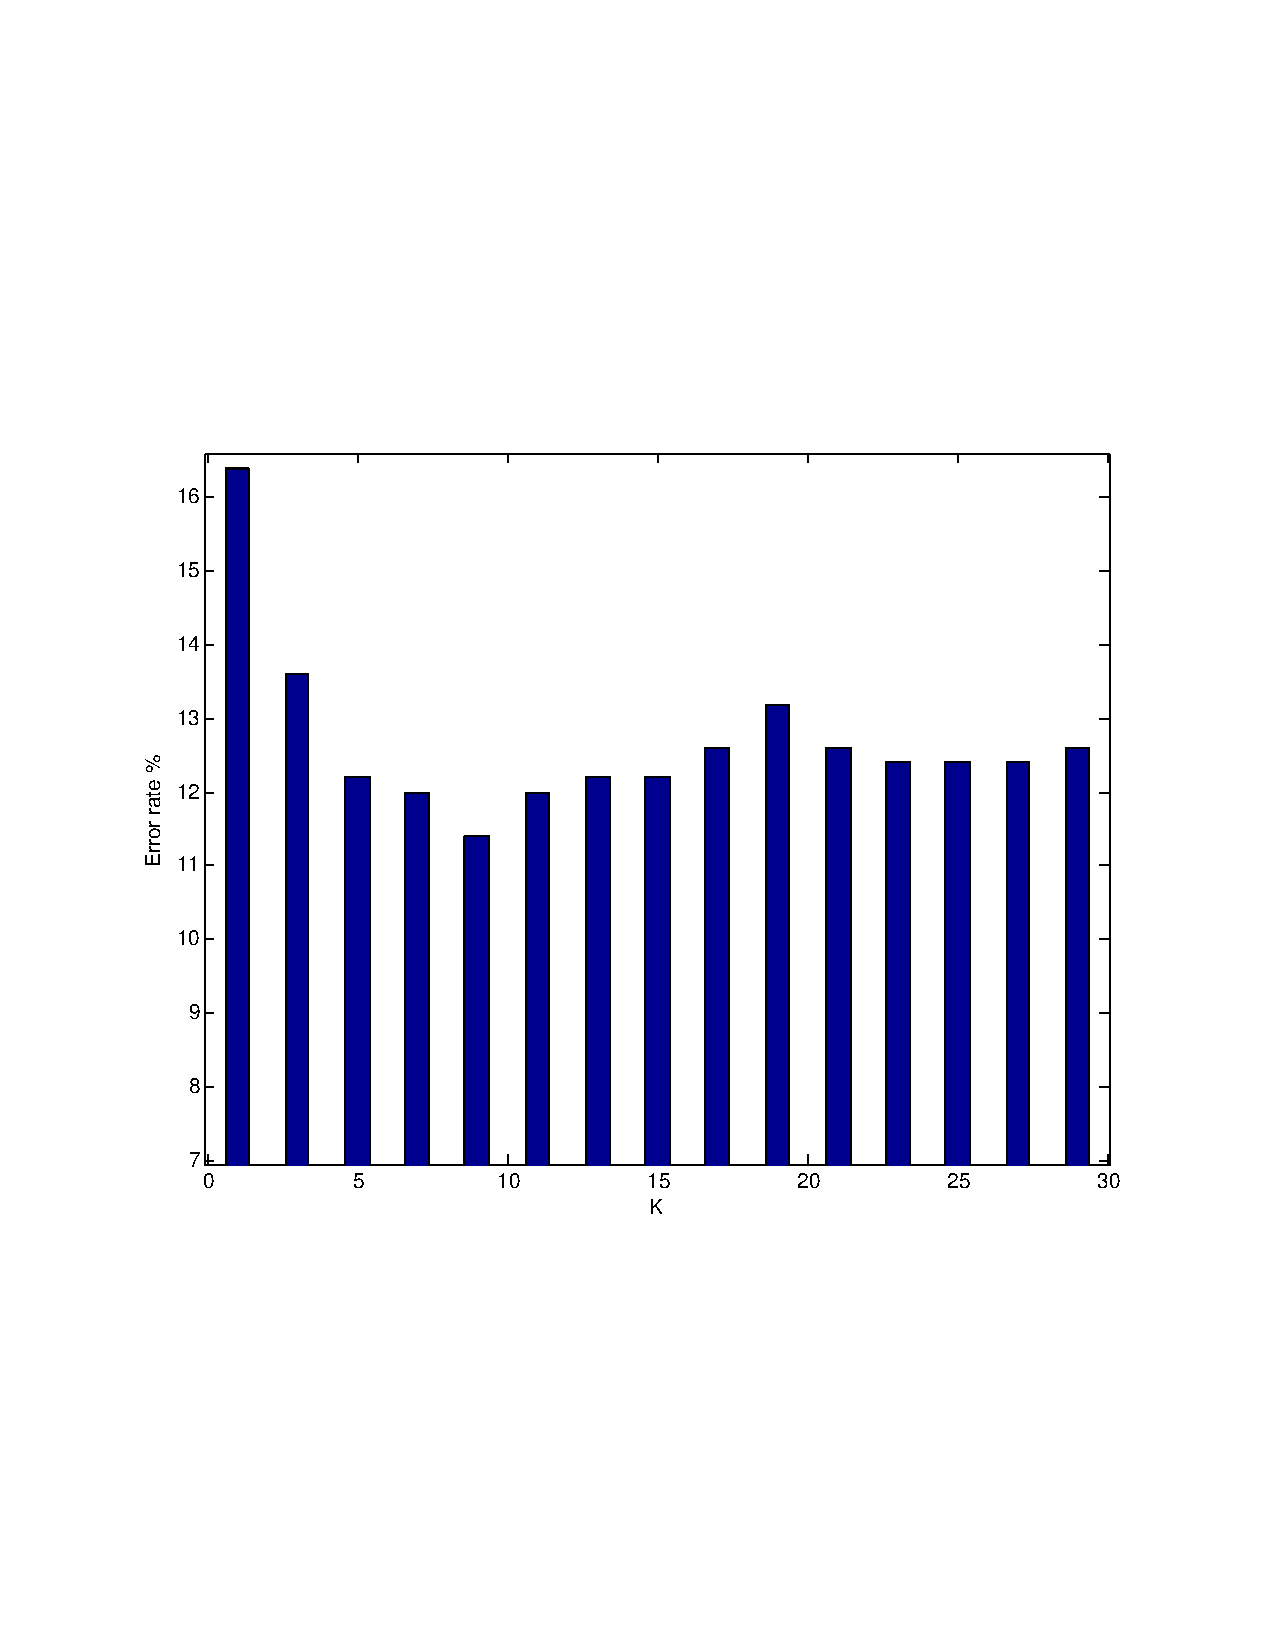
\includegraphics[trim = 0cm 7cm 0cm 7cm, clip, width=0.8\textwidth]{figures/KnnResults.pdf}
  \caption{Classification Results.}
  \label{fig:3}
\end{figure}

The value of k that we would choose is \textbf{$k=9$}, because as the figure states, for $k=9$ the \textbf{test error} reaches its \textbf{minimum} value, however, for $k>9$, an increment of the misclassification rate is detected as we increase the value of k. However, we are not able to definitely state that $k=9$ is the optimal value for k. As mentioned above, as the value of k increases, the test error is expected to decrease. This behavior does not refer to the whole range of k's tested values, but as k becomes significantly high the test error calculated increments as well. We interpreted this fact as a typical case of \textbf{overfitting}, which is \textbf{expected} to occur if the value of k becomes high enough (in this case, $k>9$).



 \section*{Exercise 3}
 \subsection*{3.1}
As described before, the problem of \textbf{overfitting} occurs while we are increasing the value of k. This may happens because either we have a model which is too complex, or the data used for training is too little. In our case, the model is relatively simple so, we should find a way to increase our training data. Here comes the solution of \textbf{cross-Validation}. Cross-Validation helps us to overcome the problem of overfitting while \textbf{expands the data used for training purposes}. In each iteration of the algorithm, a new training and test set are used, offers us more \textbf{accurate predictions} when it comes to validation. Another algorithm we could have applied, in order to increase accuracy, is \textbf{Bootstrapping} algorithm, which can lead us at least to a critical conclusion regarding the variance of the training data we are given, informing us about the possible outcome of the whole simulation. We applied Cross-Validation algorithm not only to expand our training and test data, but also to reach to a more \textbf{reliable and accurate conclusion} about the optimal value of k. 


\begin{figure}[!h]
\centering
  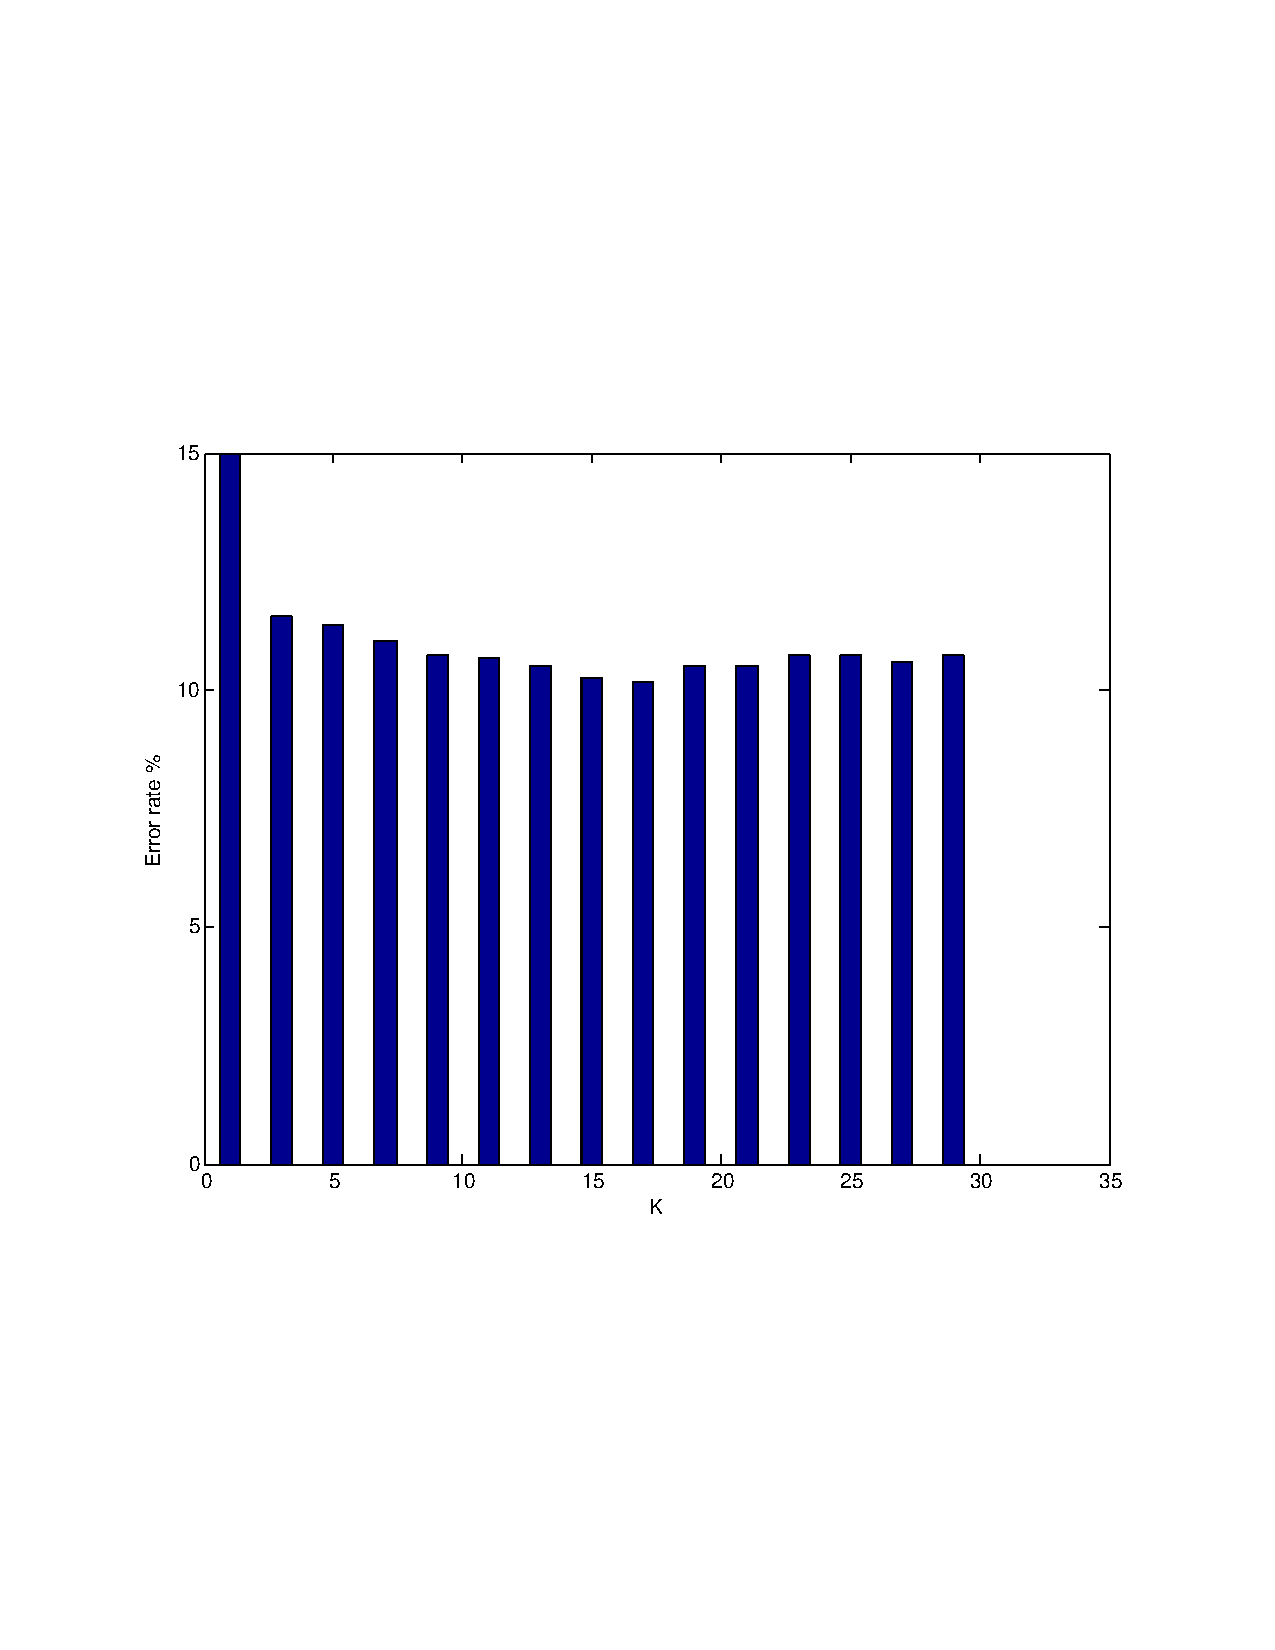
\includegraphics[trim = 0cm 7cm 0cm 7cm, clip, width=0.8\textwidth]{figures/CrossValResults.pdf}
  \caption{Results of Cross-Validation}
  \label{fig:4}
\end{figure}


\subsection*{3.2}
In the second part of exercise three we implemented Cross-Validation algorithm in order to derive more accurately an optimal value for $k$. 10-Fold Cross Validation splits data into $10$ equal subsets. In each iteration of the algorithm we use one of these subsets as the validation (test) data and the other nine subsets to train our classifier. The outcome of this implementation is presented in Figure~\ref{fig:4}. The misclassification error of the cross-validated data reaches its minimum value for $k=9$, enabling us to choose more accurately an optimal value for k variable. We chose $k=9$ as a good estimation. 


\subsection*{3.3}
This value ($k=9$) is the one that we can use in our \textbf{final classifier}, although the misclassification rate becomes minimum when $k=17$. We have chosen $k=9$ because we prefer to "sacrifice" a very small difference in the algorithm's \textbf{accuracy} in order to implement a more \textbf{simple} classificator. We estimated that a value of $k=17$ would over-smooth our classificator and make our algorithm \textbf{computationally expensive}. Cross-validation is a way to predict the accuracy of a model to a hypothetical test set when a definite test set is not available. Cross-validation algorithm is an applicable way to predict the performance of a model on a test set using your data in a way that more accurate estimation can be derived. 

\subsection*{3.4}
To compute the \textbf{test error}, we calculate the \textbf{average} misclassification reate over the 10 iterations of the 10-fold Cross-Validation algorithm. The test error computed is different in each iteration, so the \textbf{average} value gives us a good estimation of the misclassification rate. The classification error which we computed is an estimation over several experiments with different training and validation data. The use of a \textbf{validation set} is to define whether the predictions of the classification are accurate or not.

\subsection*{Further Experimentation}
To experiment further with the k-NN algorithm we applied the Cross-Validation method over a huge amount of values for the k variable. We used a set of values $k= \lbrace 1, 3, 5,\ldots, 1000 \rbrace$. In Figure~\ref{fig:5} presented the results of our experiment. We can distinguish two regions. The red colored region is the results of the k-NN algorithm when we apply it with a big value for its k variable. We can realize that giving such a huge value for the k variable results to the increase of the misclassification rate as the desicion boundaries are becoming really smooth. 

\begin{figure}[!t]
\centering
  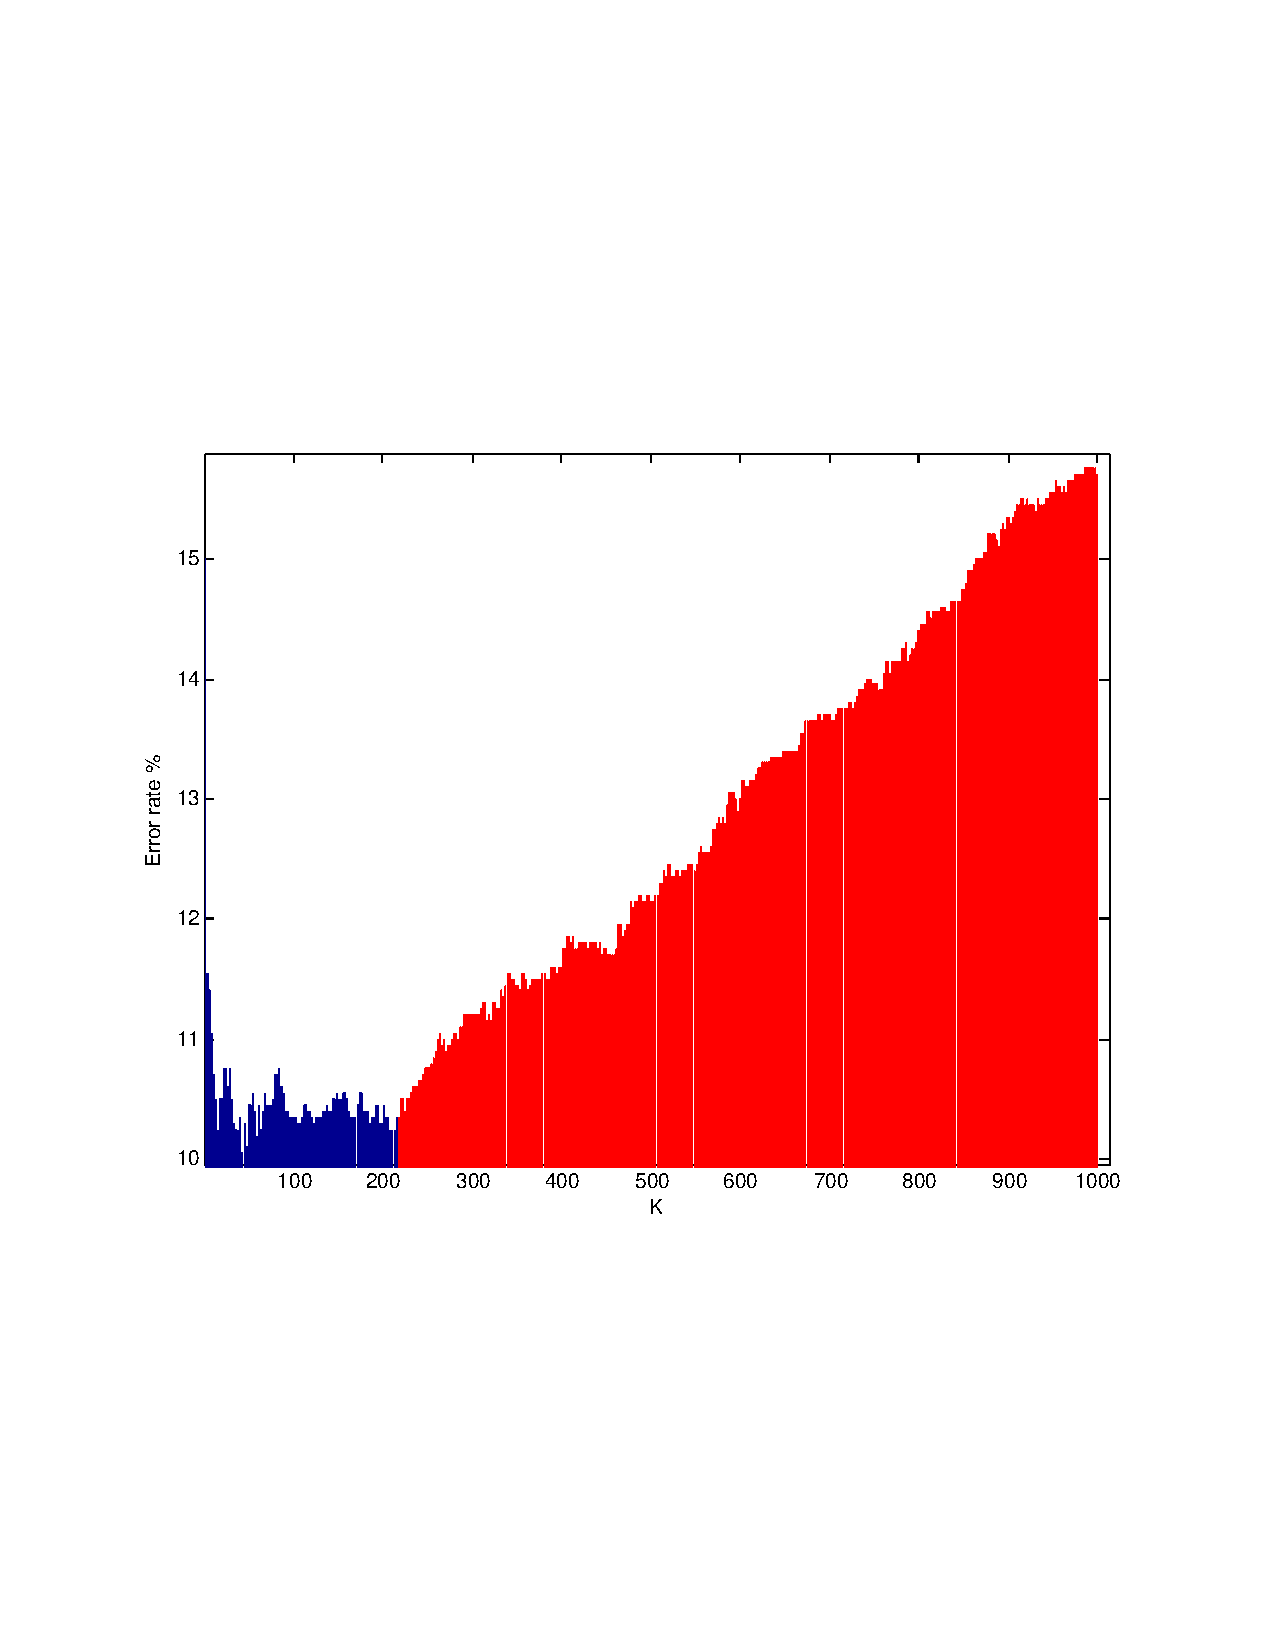
\includegraphics[trim = 0cm 7cm 0cm 7cm, clip, width=0.8\textwidth]{figures/FurtherTest.pdf}
  \caption{Further Experimentation}
  \label{fig:5}
\end{figure}

 \section*{Conclusion}
In conclusion, this project clearly helped us to understand the nature of the k-NN algorithm. Moreover, we were able to point out its advantages while facing the expected drawbacks, like the overfitting phenomenon. On the other hand we studied and implemented methods of dealing with overfitting, and thus reaching more accurate and reliable conclusions.


    \end{document}


